\documentclass[twocolumn, aps, amsmath, amssymb, nofootinbib, superscriptaddress, longbibliography, floatfix, eqsecnum, rmp]{revtex4-2}

\usepackage[pdftex]{graphicx}
\usepackage{mathrsfs}
\usepackage[colorlinks, breaklinks, urlcolor={blue}, linkcolor={red}, citecolor={blue}]{hyperref}
\usepackage{mathtools}
\usepackage[english]{babel}
\usepackage{booktabs}
\usepackage{type1cm}
\usepackage{caption}
\usepackage{url}
\usepackage{braket}
\usepackage{algorithm}
\usepackage{algpseudocodex}
\usepackage[strict]{changepage}
\usepackage{tikz}
\usepackage{tikz-3dplot}
\usepackage{pgfplots}

\pgfplotsset{compat=newest}

\usetikzlibrary{positioning, fit, calc, shadows, shadows.blur, arrows.meta, shapes.geometric, fillbetween, fadings}

%\let\oldalgorithmic\algorithmic
%\let\endoldalgorithmic\endalgorithmic
%\renewenvironment{algorithmic}
%{\begin{adjustwidth}{-1em}{}\oldalgorithmic}
%{\endoldalgorithmic\end{adjustwidth}}

\colorlet{nodeVLineColor}{blue}
\colorlet{nodeVFillColor}{cyan!20}
\colorlet{nodeULineColor}{orange}
\colorlet{nodeUFillColor}{yellow!20}
\colorlet{nodeRedLineColor}{red}
\colorlet{nodeRedFillColor}{red!20}
\colorlet{nodeGreenLineColor}{green}
\colorlet{nodeGreenFillColor}{green!20}
\colorlet{nodeBlueLineColor}{blue}
\colorlet{nodeBlueFillColor}{cyan!20}
\colorlet{nodeBlueLineColor}{blue}
\colorlet{nodeBlueFillColor}{cyan!20}
\colorlet{graphEdgeColor}{gray}
\colorlet{graphNonEdgeColor}{lightgray}
\colorlet{setDFillColor}{red!20}
\colorlet{setHFillColor}{green!20}
\colorlet{setHDFillColor}{blue!20}
\colorlet{topologyFillColor}{cyan!10}
\colorlet{blockchainDiscColor}{blue!10}
\colorlet{blockchainPendingDiscColor}{red!10}
\colorlet{redHighlightColor}{red!80}
\colorlet{blueHighlightColor}{blue!80}

\tikzset{
	genericStyle/.style = {
		every node/.style = {circle, draw, minimum size=2em}, >=latex
	}
}

\tikzset{
	myShadow/.style = {
		blur shadow = {shadow blur steps=5, shadow xshift=0.15em, shadow yshift=-0.1em}
	}
}

\tikzset{
	myLightShadow/.style = {
		blur shadow = {shadow blur steps=5, shadow xshift=0.1em, shadow yshift=-0.066em}
	}
}

\tikzset{
	nodeUStyle/.style = {
		draw=nodeULineColor, fill=nodeUFillColor, myShadow
	}
}

\tikzset{
	nodeVStyle/.style = {
		draw=nodeVLineColor, fill=nodeVFillColor, myShadow
	}
}

\tikzset{
	nodeGrayStyleC/.style = {
		draw=gray, fill=gray!20, myShadow
	}
}

\tikzset{
	nodeGrayStyle/.style = {
		draw=black, fill=gray!20, myShadow
	}
}

\tikzset{
	nodeLightGrayStyle/.style = {
		draw=gray, fill=lightgray!20, myShadow
	}
}

\tikzset{
	nodeRedStyle/.style = {
		draw=nodeRedLineColor, line width=0.25, line cap=round, fill=nodeRedFillColor, myLightShadow
	}
}

\tikzset{
	nodeBlueStyle/.style = {
		draw=nodeBlueLineColor, line width=0.25, line cap=round, fill=nodeBlueFillColor
	}
}

\tikzset{
	graphEdgeStyle/.style = {
		draw=graphEdgeColor, line width=1, line cap=round
	}
}
	
\tikzset{
	graphNonEdgeStyle/.style = {
		draw=graphNonEdgeColor, opacity=0.25, line width=1, line cap=round
	}
}

\tikzset{
	graphRedEdgeStyle/.style = {
		draw=red, opacity=0.5, line width=1.5, line cap=round
	}
}

\tikzset{
	graphLightRedEdgeStyle/.style = {
		draw=nodeRedLineColor, opacity=0.15
	}
}

\tikzset{
	graphBlueEdgeStyle/.style = {draw=blue!50, line width=0.5}
}

\frenchspacing
    
\captionsetup[figure]{margin=0pt, font=small, labelfont=bf, labelsep=endash, justification=centerlast, labelsep=colon}
\captionsetup[algorithm]{margin=0pt, font=small, labelfont=bf, labelsep=endash, justification=centerlast, labelsep=colon}
    
\begin{document}

\title{Quantum consensus networks}

\author{Peter P. Rohde}
\affiliation{BTQ Technologies}

\maketitle

%\section{Quantum consensus networks} \label{sec:QCN}
Quantum consensus networks (QCNs) have quantum-enabled nodes, whose goal it is to form consensus on the generation of certifiable quantum randomness, an important resource in cryptography and numerous other applications.

As quantum hardware is costly compared to classical hardware it is expected that few networks will be quantum-enabled. However, they may exploit the quantum randomness provided by dedicated QCNs acting as \emph{quantum random oracles} to inject entropy into their own global keys using \emph{entropy addition}, effectively enabling classical DCNs to achieve quantum random consensus assignment.

We consider two approaches for quantum random number generation (QRNG):
\begin{itemize}
	\item Quantum key distribution (QKD): requires quantum communication but no quantum computation.
	\item Interactive proofs of quantumness: require quantum computation but no quantum communication.
\end{itemize}

As these are two-party protocols, every instance may be associated with a graph edge between the respective nodes. Random numbers associated with edges may be spoofed if both nodes collude, bypassing the need for expensive quantum resources. However, so long as at least one contributing QRN is genuine, combining them under bit-wise XOR yields a collective QRN source.

Independent of the underlying two-party QRNG protocol, QCNs operate as follows:
\begin{enumerate}
	\item All nodes execute two-party QRNG with all other nodes, a total of $n(n-1)$ QRNG rounds.
	\item All $n$ nodes commit their versions of their QRNG outcomes with all other $n-1$ nodes.
	\item A corresponding \emph{compliance graph} is implied by the committed data. This may be realised by any entity observing the published data.
	\item A graph reduction algorithm eliminates  graph edges associated with inconsistent QRNG outcomes, followed by eliminating nodes not connected by a majority of edges.
	\item The resultant graph is a unique fully-connected subgraph representing the unanimous-majority outcome.
\end{enumerate}

%Structure:
%
%* Implied voting rules (general then specific, symmetric vs asymmetric).
%
%* Quantum random oracles (public).
%
%* Secret shared randomness (with encryption).
%
%* Specific implementations: E91 QKD, BB84 QKD, IPQ.
%
%-

%Choosing a cyclic graph spanning all nodes, $C_n$, creates a proof-chain where the existence of a single honest player guarantees the existence of a single honest edge.

%* Same as above, but now the reported measurement outcomes are utilised as the random source, enabling quantum-random subsets.
%
%* Under randomised neighbours ff a prover node is compromised the probability it's neighbouring verifier is comprised, thereby enabling shortcutting, is:
%* P=(rN-1)/N = r-1/N (P=r for large N)
%* This proportion of adversarial nodes can bypass work in proof-of-quantumness.
%* Under collusion amongst compromised nodes:
%* Only last prover in prover-graph forced to comply: P=1/N (P=0 for large N)
%
%Directed node graph constitutes the prover graph, oppositely-directed the verifier graph.
%The prover graph is $C_n$ directed one way, the verifier graph the other.
%
%Indices provided by the global hash key define a random, directed, cyclic graph, where node i acts as verifier for node i+1 and prover to node i-1. Randomised ordering ensures the probability a neighbour is compromised is uniformly r. If this ordering could be manipulated conspiring nodes could assemble themselves into a contiguous linear subgraph where only the final prover is forced to honestly comply with the proof. The other dishonest nodes can exchange secrets to manufacture legitimate proofs of quantumness without the cost of executing the respective quantum computation. While this does not impact the integrity of the established global key, it enables bypassing the costs. Scales as 1/n cost. Not a security consideration, but one of equity. Randomised ordering enforces cost reduction of r. While inhibiting the ability to bypass cost of quantum computation is enforced by hash-randomness, the established global key seeding the allocation of random subsets is quantum-random.
%
%A fixed cycle therefore upholds quantum-random subset allocation but compromises the ability to ensure r-fairness in bypassed quantum computational cost. Taking the participating set of nodes ordered by their public keys to define a fixed cyclic graph. Randomised ordering requires point-to-point connectivity between all nodes, requiring the ability to independently route $O(n^2)$ connections. Static ordering reduces this to $O(n)$. Both exhibit $O(n)$ communications complexity and ensure secure quantum-randomness.

%\subsection{Entropy sources: quantum vs. classical}
%
%* Entropy rate
%\begin{align}
%	H(\mathcal{X}) = \lim_{n\to\infty} H(\mathcal{X}_n | \mathcal{X}_{n-1},\dots,\mathcal{X}_1),
%\end{align}
%where $H(X|Y)$ is the conditional entropy of $X$ given knowledge of $Y$.
%
%TO DO:
%
%* What is quantum random vs classical random.
%
%* Correlations over repeats?
%
%For iid (quantum)
%\begin{align}
%	H(\mathcal{X}) = H(\mathcal{X}_n)
%\end{align}

\section{Entropy addition} \label{sec:entropy_add}

The bit-wise XOR operator is a strictly non-entropy-decreasing function. For binary random variables,
\begin{align}
	\mathcal{X}_i\to\{0,1\},
\end{align}
with probability distributions,
\begin{align}
	\mathcal{X}_i \sim \mathrm{Ber}(p_i):\, p_i=p_i(0)=1-p_i(1),
\end{align}
the individual binary Shannon entropies are given by,
\begin{align}
	H_2(\mathcal{X}_i) = -p_i\log_2 p_i - (1-p_i)\log_2(1-p_i),
\end{align}
where,
\begin{align}
	0 \leq H_2(\cdot) \leq 1,
\end{align}
the entropy of the random variable given by their bit-wise XOR,
\begin{align}
	\mathcal{X} = \bigoplus_i \mathcal{X}_i,
\end{align}
is lower-bounded by the maximum entropy of the contributing random variables,
\begin{align}
	\max_i(\{H_2(\mathcal{X}_i)\}) \leq H_2(\mathcal{X}) \leq 1.
\end{align}

Hence, a random source derived from multiple sources via entropy addition is at least as random as any of them. Consequently, if any single contributing source is a genuine QRNG, so too will be their the combined source.

Note that hash functions do not exhibit the entropy addition property of the bitwise XOR operation and cannot be employed in this context.

\section{Quantum random oracles} \label{sec:quantum_rand_oracles}

Let $\mathcal{O}(t)$ denote a dynamic set of contributing random oracles at  time $t$. We define a collective random bitstream,
\begin{align}
	\mathcal{X}_\mathcal{O}(t) = \bigoplus_{i\in\mathcal{O}(t)} \mathcal{X}_i(t),
\end{align}
whose combined entropy is bounded by,
\begin{align}
	\max_{i\in\mathcal{O}}(\{H_2(\mathcal{X}_i)\}) \leq H_2(\mathcal{X}_{\mathcal{O}}) \leq 1.
\end{align}

A classical DCN may observe a QRNG oracle and add its entropy $\mathcal{X}_\mathcal{O}$ to its own global key. For this to be secure it is required that the DCN's own global key, $\mathcal{X}_\mathcal{N}$, be committed prior to the availability of the external entropy source,
\begin{align}
	{\mathcal{\tilde X}}_\mathcal{N}(t+\tau) = \mathcal{X}_\mathcal{N}(t) \oplus \mathcal{X}_\mathcal{O}(t+\tau),
\end{align}
where ${\mathcal{\tilde X}}_\mathcal{N}$ is the network's oracle-modulated global key, and \mbox{$\tau>0$} is a pre-agreed future point in time, subsequent to commitment of the networks initially established global key, $\mathcal{X}_\mathcal{N}$.

\begin{figure}
\begin{center}
	\tikzset{
    blueGlow/.style = {
            draw=blue!70, fill=blue!40, circular glow={fill=blue!40, shadow scale=1.25, shadow blur steps=5
                }
        }
}

\tikzset{
    myShadow/.style = {
            blur shadow = {shadow blur steps=5, shadow xshift=0.15em, shadow yshift=-0.1em}
        }
}

\tikzset{
    blueShadow/.style = {
            draw=blue!40, line width=2, drop shadow = {color=blue, shadow blur steps=5, shadow xshift=0.15em, shadow yshift=-0.1em}
        }
}

\tikzset{
    redShadow/.style = {
            draw=red!40, line width=2.5, drop shadow = {color=blue, shadow blur steps=5, shadow xshift=0.15em, shadow yshift=-0.1em}
        }
}

\tikzset{
    blockchainCol/.pic={
            \tikzset{blockchainCol/.cd,#1}
            \def\pv##1{\pgfkeysvalueof{/tikz/blockchainCol/##1}}

            \fill[fill=topologyFillColor] (-\myWidth,0) rectangle (\myWidth,4*\discSep);

            \node[draw=none, fill=blockchainDiscColor, ellipse, minimum width=\myWidth, minimum height=\myHeight, myShadow] (node0) at (0,0) {};
            \draw[darkgray] (-\myWidth,0) arc [start angle=0, end angle=-180, x radius=-\myWidth, y radius =\myHeight];
            \draw[gray, dashed] (-\myWidth,0) arc [start angle=0, end angle=180, x radius=-\myWidth, y radius =\myHeight];

            \node[draw=none, fill=blockchainDiscColor, ellipse, minimum width=\myWidth, minimum height=\myHeight] (node1) at (0,\discSep) {};
            \draw[darkgray] (-\myWidth,\discSep) arc [start angle=0, end angle=-180, x radius=-\myWidth, y radius =\myHeight];
            \draw[gray, dashed] (-\myWidth,\discSep) arc [start angle=0, end angle=180, x radius=-\myWidth, y radius =\myHeight];

            \node[draw=none, fill=blockchainDiscColor, ellipse, minimum width=\myWidth, minimum height=\myHeight] (node2) at (0,2*\discSep) {};
            \draw[darkgray] (-\myWidth,2*\discSep) arc [start angle=0, end angle=-180, x radius=-\myWidth, y radius =\myHeight];
            \draw[gray, dashed] (-\myWidth,2*\discSep) arc [start angle=0, end angle=180, x radius=-\myWidth, y radius =\myHeight];

            \node[draw=none, fill=blockchainDiscColor, ellipse, minimum width=\myWidth, minimum height=\myHeight] (node2) at (0,3*\discSep) {};
            \draw[darkgray] (-\myWidth,3*\discSep) arc [start angle=0, end angle=-180, x radius=-\myWidth, y radius =\myHeight];
            \draw[gray, dashed] (-\myWidth,3*\discSep) arc [start angle=0, end angle=180, x radius=-\myWidth, y radius =\myHeight];

            \node[draw=none, fill=blockchainDiscColor, ellipse, minimum width=\myWidth, minimum height=\myHeight] (node2) at (0,4*\discSep) {};
            \draw[darkgray] (-\myWidth,4*\discSep) arc [start angle=0, end angle=-180, x radius=-\myWidth, y radius =\myHeight];
            \draw[darkgray] (-\myWidth,4*\discSep) arc [start angle=0, end angle=180, x radius=-\myWidth, y radius =\myHeight];

            \draw[blueShadow, line width=2] (0,0) -- (0,4*\discSep);

            \draw[blueGlow] (0,0) circle (\ballRadius);
            \draw[blueGlow] (0,\discSep) circle (\ballRadius);
            \draw[blueGlow] (0,2*\discSep) circle (\ballRadius);
            \draw[blueGlow] (0,3*\discSep) circle (\ballRadius);
            \draw[blueGlow] (0,4*\discSep) circle (\ballRadius);

            \draw[darkgray] (-\myWidth,0) -- (-\myWidth,4*\discSep);
            \draw[darkgray] (\myWidth,0) -- (\myWidth,4*\discSep);
        }
}

\begin{tikzpicture}[genericStyle, scale=0.5]
    \def\myWidth{6em}
    \def\myHeight{2.5em}
    \def\discSep{2}
    \def\ballRadius{0.15}
    \def\xadj{0.1}
    \def\yoff{0.75}
    \def\xoff{6.5}

    \colorlet{lineBaseCol}{red}
    \pic[scale=0.5] at (0,0) {blockchainCol};
    \colorlet{lineBaseCol}{blue}
    \pic[scale=0.5] at (-\xoff,-\yoff) {blockchainCol};
    \pic[scale=0.5] at (\xoff,-\yoff) {blockchainCol};

    \draw[->, redShadow, line cap=round, opacity=0.7] (\xadj,4*\discSep) -> (\xoff-\xadj,3*\discSep-\yoff);
    \draw[blueGlow] (0,3*\discSep) circle (\ballRadius);
    \draw[blueGlow] (0,4*\discSep) circle (\ballRadius);

    \def\labelY{4.8*\discSep}
    \node[draw=none, text=black] at (0,\labelY) {$\mathcal{X}_\mathcal{O}$(t)};
    \node[draw=none, text=black] at (-\xoff,\labelY-\yoff) {$\mathcal{X}_\mathcal{N}(t)$};
    \node[draw=none, text=black] at (\xoff,\labelY-\yoff) {$\mathcal{X}_\mathcal{N}(t) \oplus \mathcal{X}_\mathcal{O}(t+\tau)$};

    \draw[darkgray] (-\myWidth+\xadj,4*\discSep) arc [start angle=0, end angle=-180, x radius=-\myWidth, y radius =\myHeight];
    \draw[darkgray] (-\myWidth+\xadj,0) -- (-\myWidth,4*\discSep);
\end{tikzpicture}

\caption{\textbf{Quantum random oracles.} A classical DCN establishing hash-based secure random source $\mathcal{X}_\mathcal{N}(t)$, where $t$ denotes time, may add entropy from a QCN acting as oracle for quantum random source $\mathcal{X}_\mathcal{O}(t)$. To maintain security $\mathcal{X}_\mathcal{N}$ must be established in advance of $\mathcal{X}_\mathcal{O}$, achieved by adding entropy from a QRN outcome at pre-agreed future time $t+\tau$, $\tilde{\mathcal{X}}_\mathcal{N}(t) = \mathcal{X}_\mathcal{N}(t) \oplus \mathcal{X}_\mathcal{O}(t+\tau)$.}
\label{fig:QRNG_oracle}
\end{center}
\end{figure}

\section{Quantum key distribution (QKD)} \label{sec:QKD}

Quantum key distribution (QKD) \cite{BB84, E91} enables the secure establishment of shared randomness between two parties with information theoretic security. While ordinarily utilised for secret key exchange, here we exploit not the secrecy of shared randomness but its inability to be spoofed under honest execution of the protocol.

Assuming the existence of a quantum internet \cite{RohdeQI} capable of arbitrary point-to-point entanglement routing, all node-pairs $(i,j)$ have access to an indefinite supply of maximally-entangled Bell pairs,
\begin{align}
	\ket{\Psi}_{i,j} = \frac{1}{\sqrt{2}}(\ket{0}_i\ket{0}_j+\ket{1}_i\ket{1}_j),
\end{align}
requiring full $O(n^2)$ quantum communications connectivity.

For the $n$th copy of $\ket{\Psi}_{i,j}$ both nodes independently and privately choose measurement bases,
\begin{align}
	b_i(n),b_j(n)\in\{0,1\},
\end{align}
where \mbox{$b=0$} denotes the Pauli-$Z$ basis and $b=1$ the Pauli-$X$ basis, and record their associated measurement outcomes,
\begin{align}
	m_i(n),m_j(n)\in\{0,1\}.
\end{align}
The subset of measurement outcomes where both parties operate in the same basis defines a shared random bit-string,
\begin{align}
	s_{i,j} = \{m(n)\,|\, b_i(n)=b_j(n)\}_n.
\end{align}
These post-selected bit-strings correspond identically to those provided by the E91 \cite{E91} QKD protocol. The BB84 protocol \cite{BB84} can be similarly employed with the interpretational difference that for one party $b$ and $m$ denote encoding, for the other measurement.

Physical and implementation errors reduce the otherwise perfect measurement correlations between nodes measuring in the same basis resulting in inconsistent shared strings. However, privacy amplification \cite{PrivacyAmp} may be used to reduce an imperfect random bit-string to a shorter one with higher entropy using classical post-processing.

%Using the existing hash-based global key we assign nodes to a randomly-ordered cyclic graph $C_n$, where we assume the availability of arbitrary point-to-point QKD links between all nodes in the network. For every edge in $C_n$ the two connecting nodes implement a QKD protocol, whose outcome is associated with the respective graph edge, shown in Fig.~\ref{fig:proof_chains}.
%
%The quantum-random global key is established by XORing all compliant QRNs as per Eq.~\eqref{eq:global_K}. Since cyclic graphs are connected, the existence of any honest nodes guarantees that at least one edge was honestly executed, sufficient to uphold the integrity of the established key.

%To introduce QKD-derived global keys to the protocol we introduce additional synchronous steps. Following the \textsc{Accept} stage of the classical DCN protocol, nodes are required to commit QRN strings obtained in accordance with the randomised $C_n$ graph. The \textsc{Compliance} stage of the protocol now additionally requires all committed QKD strings to pass a legitimacy test for compliance.

%In the case of entanglement-based E91 networks, both nodes measure their received qubits from distributed Bell-pairs randomly in the $X$ or $Z$ bases, where the number of samples taken $n$ ensures the post-processed QRN bit-string has sufficient length. Both sides commit their sequence of measurement bases ($b\in\{0,1\}^n$) and outcomes ($m\in\{0,1\}^n$). Once revealed, the subset of values where both parties operated in the same basis defines their pairwise shared source of randomness,
%\begin{align}
%	K_{A,B} = \{m(i)\,|\, b_A(i)=b_B(i)\}.
%\end{align}

\begin{figure}[!htb]
	\resizebox{0.32\columnwidth}{!}{
  \begin{tikzpicture}[genericStyle, every node/.style={circle, draw, minimum size=1.8em, text width=1em, align=center, inner sep=0pt}]
    \def\UVsep{2.5em}
    \def\colSep{3em}
    \def\rowSep{1.2em}
    \def\hStep{0.7em}

    % Radius of the circle
    \def\radius{5em}
    \def\numnodes{8}
    \def\degree{360/\numnodes}

    % Draw dummy nodes
    \foreach \x in {1,...,\numnodes} {
        \node[draw=none] (node\x) at (\x*\degree+0.5*\degree+180:\radius) {};
      }

    % Draw gray lines
    \foreach \x in {1,...,\numnodes} {
        \foreach \y in {\x,...,\numnodes} {
            \pgfmathparse{(\y>\x+1) && (1-(\x==1 && \y==\numnodes)) ? 1 : 0}
            \ifnum \pgfmathresult=1
              \draw[graphNonEdgeStyle] (node\x) -- (node\y);
            \fi
          }
      }
    \node[draw, circle, minimum size=2*\radius, graphNonEdgeStyle] at (0,0) {};

    % Draw red lines
    \foreach \x in {1,...,\numnodes} {
        \foreach \y in {\x,...,\numnodes} {
            \pgfmathparse{(\y>\x+1) && (1-(\x==1 && \y==\numnodes)) ? 1 : 0}
            \ifnum \pgfmathresult=1
              \draw[graphRedEdgeStyle] (node\x) -- (node\y);
            \fi
          }
      }
    \node[draw, circle, minimum size=2*\radius, graphRedEdgeStyle] at (0,0) {};

    % Visible nodes
    \foreach \x in {1,...,\numnodes} {
        \ifnum\x=1
          \node[nodeConsensusStyle] (node\x) at (\x*\degree+0.5*\degree+180:\radius) {\large $i$};
        \else
          \ifnum\x=2
            \node[nodeConsensusStyle, text=black] (node\x) at (\x*\degree+0.5*\degree+180:\radius) {\large $j$};
          \else
            \node[nodeConsensusStyle] (node\x) at (\x*\degree+0.5*\degree+180:\radius) {};
          \fi
        \fi
      }

    % Labels
    \coordinate (mid) at ($(node1.east)!0.5!(node2.west) + (0,-2.2em)$);
    \node[draw=none, rectangle, text width=8em] () at (mid) {\large $s_{i,j}=\mathrm{QKD}_{i,j}$};
    \node[draw=none, rectangle, right=0.5em of node5, text=red] () {\large $K_n$};
  \end{tikzpicture}
}
\hfill
\resizebox{0.32\columnwidth}{!}{
  \begin{tikzpicture}[genericStyle, every node/.style={circle, draw, minimum size=1.8em, text width=1em, align=center, inner sep=0pt}]
    \def\UVsep{2.5em}
    \def\colSep{3em}
    \def\rowSep{1.2em}
    \def\hStep{0.7em}

    % Radius of the circle
    \def\radius{5em}
    \def\numnodes{8}
    \def\degree{360/\numnodes}

    % Draw dummy nodes
    \foreach \x in {1,...,\numnodes} {
        \node[draw=none] (node\x) at (\x*\degree+0.5*\degree+180:\radius) {};
      }

    % Draw gray lines
    \foreach \x in {1,...,\numnodes} {
        \foreach \y in {\x,...,\numnodes} {
            \pgfmathparse{(\y>\x+1) && (1-(\x==1 && \y==\numnodes)) ? 1 : 0}
            \ifnum \pgfmathresult=1
              \draw[graphNonEdgeStyle] (node\x) -- (node\y);
            \fi
          }
      }
    \node[draw, circle, minimum size=2*\radius, graphNonEdgeStyle] at (0,0) {};

    % Draw red lines
    \foreach \x in {1,...,\numnodes} {
        \foreach \y in {\x,...,\numnodes} {
            \pgfmathparse{(\y>\x+1) && (1-(\x==1 && \y==\numnodes)) ? 1 : 0}
            \ifnum \pgfmathresult=1
              \pgfmathparse{(\x==1 && \y==3) || (\x==1 && \y==4) || (\x==3 && \y==5) || (\x==3 && \y==6) || (\x==3 && \y==7) || (\x==4 && \y==6) || (\x==4 && \y==8) ? 1 : 0}
              \ifnum \pgfmathresult=0
                \draw[graphRedEdgeStyle] (node\x) -- (node\y);
              \fi
            \fi
          }
      }
    \node[draw, circle, minimum size=2*\radius, graphRedEdgeStyle] at (0,0) {};

    % Visible nodes
    \foreach \x in {1,...,\numnodes} {
        \ifnum\x=1
          \node[nodeConsensusStyle, text=black] (node\x) at (\x*\degree+0.5*\degree+180:\radius) {\large $i$};
        \else
          \ifnum\x=2
            \node[nodeConsensusStyle, text=black] (node\x) at (\x*\degree+0.5*\degree+180:\radius) {\large $j$};
          \else
            \node[nodeConsensusStyle] (node\x) at (\x*\degree+0.5*\degree+180:\radius) {};
          \fi
        \fi
      }

    % Labels
    \coordinate (mid) at ($(node1.east)!0.5!(node2.west) + (0,-2.2em)$);
    \node[draw=none, rectangle, text width=10em] () at (mid) {\large $e_{i,j}=f_\mathrm{QKD}(s_{i,j})$};
  \end{tikzpicture}
}
\hfill
\resizebox{0.32\columnwidth}{!}{
  \begin{tikzpicture}[genericStyle, every node/.style={circle, draw, minimum size=1.8em, text width=1em, align=center, inner sep=0pt}]
    \def\UVsep{2.5em}
    \def\colSep{3em}
    \def\rowSep{1.2em}
    \def\hStep{0.7em}

    % Radius of the circle
    \def\radius{5em}
    \def\numnodes{8}
    \def\degree{360/\numnodes}

    % Draw dummy nodes
    \foreach \x in {1,...,\numnodes} {
        \node[draw=none] (node\x) at (\x*\degree+0.5*\degree+180:\radius) {};
      }

    % Draw gray lines
    \foreach \x in {1,...,\numnodes} {
        \foreach \y in {\x,...,\numnodes} {
            \pgfmathparse{(\y>\x+1) && (1-(\x==1 && \y==\numnodes)) ? 1 : 0}
            \ifnum \pgfmathresult=1
              \draw[graphNonEdgeStyle] (node\x) -- (node\y);
            \fi
          }
      }
    \node[draw, circle, minimum size=2*\radius, graphNonEdgeStyle] at (0,0) {};

    % Draw red lines
    \draw[graphRedEdgeStyle] (node1) -- (node2);
    \draw[graphRedEdgeStyle] (node1) -- (node5);
    \draw[graphRedEdgeStyle] (node1) -- (node6);
    \draw[graphRedEdgeStyle] (node1) -- (node7);
    \draw[graphRedEdgeStyle] (node1) -- (node8);
    \draw[graphRedEdgeStyle] (node2) -- (node5);
    \draw[graphRedEdgeStyle] (node2) -- (node6);
    \draw[graphRedEdgeStyle] (node2) -- (node7);
    \draw[graphRedEdgeStyle] (node2) -- (node8);
    \draw[graphRedEdgeStyle] (node5) -- (node6);
    \draw[graphRedEdgeStyle] (node5) -- (node7);
    \draw[graphRedEdgeStyle] (node5) -- (node8);
    \draw[graphRedEdgeStyle] (node6) -- (node7);
    \draw[graphRedEdgeStyle] (node6) -- (node8);
    \draw[graphRedEdgeStyle] (node7) -- (node8);

    % Visible nodes
    \foreach \x in {1,...,\numnodes} {
        \ifnum\x=3
          \node[nodeConsensusStyle] (node\x) at (\x*\degree+0.5*\degree+180:\radius) {};
        \else
          \ifnum\x=4
            \node[nodeConsensusStyle] (node\x) at (\x*\degree+0.5*\degree+180:\radius) {};
          \else
            \node[nodeConsensusStyle] (node\x) at (\x*\degree+0.5*\degree+180:\radius) {};
          \fi
        \fi
      }

    % Labels
    \coordinate (midK) at ($(node2)!0.5!(node5)$);
    \node[draw=none, right=-0.25em of midK, text=red] {\large $K_{|\mathrm{QKD}|}$};

    \coordinate (mid) at ($(node1.east)!0.5!(node2.west) + (0,-2.2em)$);
    \node[draw=none, rectangle, text width=10em] () at (mid) {\large $\mathcal{G}_\mathrm{QKD}=K_{|\mathrm{QKD}|}$};
  \end{tikzpicture}
}
	%	\resizebox{0.49\columnwidth}{!}{
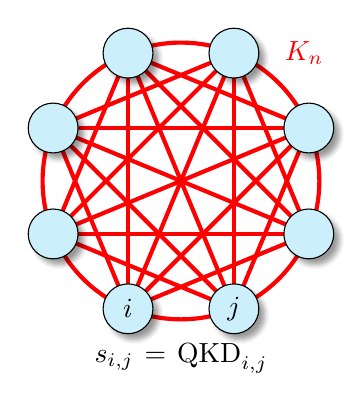
\begin{tikzpicture}[every node/.style={circle, draw, minimum size=1.8em, text width=1em, align=center, inner sep=0pt}, >=latex,
    myshadow/.style={
        blur shadow={shadow blur steps=5}
    }
]
    \def\UVsep{2.5em}
    \def\colSep{3em}
    \def\rowSep{1.2em}
    \def\hStep{0.7em}

    \definecolor{verylightgray}{rgb}{0.9, 0.9, 0.9}
    \colorlet{verylightorange}{orange!20}
    \colorlet{verylightblue}{cyan!20}

 % Radius of the circle
  \def\radius{5em}
  \def\numnodes{8}
  \def\degree{360/\numnodes}

  % Draw dummy nodes
  \foreach \x in {1,...,\numnodes} {
        \node[draw=none] (node\x) at (\x*\degree+0.5*\degree+180:\radius) {};
  }

  % Draw gray lines
  \foreach \x in {1,...,\numnodes} {
    \foreach \y in {\x,...,\numnodes} {
      \pgfmathparse{(\y>\x+1) && (1-(\x==1 && \y==\numnodes)) ? 1 : 0}
        \ifnum \pgfmathresult=1
            \draw[-,blue!20, opacity=0.5,line width=1.5,line cap=round] (node\x) -- (node\y);
        \fi
    }
  }
 \node[draw, circle, minimum size=2*\radius,blue!20, opacity=0.5,line width=1.5,line cap=round] at (0,0) {};

  % Draw red lines
  \foreach \x in {1,...,\numnodes} {
    \foreach \y in {\x,...,\numnodes} {
      \pgfmathparse{(\y>\x+1) && (1-(\x==1 && \y==\numnodes)) ? 1 : 0}
        \ifnum \pgfmathresult=1
            \draw[-,red,line width=1.5,line cap=round] (node\x) -- (node\y);
        \fi
    }
  }
 \node[draw, circle, minimum size=2*\radius,red,line width=1.5,line cap=round] at (0,0) {};

  % Visible nodes
  \foreach \x in {1,...,\numnodes} {
    \ifnum\x=1
        \node[circle,fill=verylightblue,myshadow] (node\x) at (\x*\degree+0.5*\degree+180:\radius) {$i$};
    \else
       \ifnum\x=2
            \node[circle,fill=verylightblue,myshadow] (node\x) at (\x*\degree+0.5*\degree+180:\radius) {$j$};
        \else
            \node[circle,fill=verylightblue,myshadow] (node\x) at (\x*\degree+0.5*\degree+180:\radius) {};
        \fi
    \fi
  }

  % Labels
  \coordinate (mid) at ($(node1.east)!0.5!(node2.west) + (0,-1.8em)$); 
  \node[draw=none, rectangle, text width=8em] () at (mid) {$s_{i,j}=\mathrm{QKD}_{i,j}$};
  \node[draw=none,rectangle, right=0.5em of node5,text=red] () {$K_n$};
\end{tikzpicture}
}
\hfill
\resizebox{0.49\columnwidth}{!}{
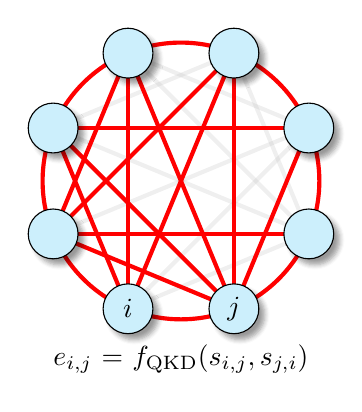
\begin{tikzpicture}[every node/.style={circle, draw, minimum size=1.8em, text width=1em, align=center, inner sep=0pt}, >=latex,
    myshadow/.style={
        blur shadow={shadow blur steps=5}
    }
]
    \def\UVsep{2.5em}
    \def\colSep{3em}
    \def\rowSep{1.2em}
    \def\hStep{0.7em}

    \definecolor{verylightgray}{rgb}{0.9, 0.9, 0.9}
    \colorlet{verylightorange}{orange!20}
    \colorlet{verylightblue}{cyan!20}

 % Radius of the circle
  \def\radius{5em}
  \def\numnodes{8}
  \def\degree{360/\numnodes}

  % Draw dummy nodes
  \foreach \x in {1,...,\numnodes} {
        \node[draw=none] (node\x) at (\x*\degree+0.5*\degree+180:\radius) {};
  }

  % Draw gray lines
  \foreach \x in {1,...,\numnodes} {
    \foreach \y in {\x,...,\numnodes} {
      \pgfmathparse{(\y>\x+1) && (1-(\x==1 && \y==\numnodes)) ? 1 : 0}
        \ifnum \pgfmathresult=1
            \draw[-,lightgray, opacity=0.25,line width=1.5,line cap=round] (node\x) -- (node\y);
        \fi
    }
  }
 \node[draw, circle, minimum size=2*\radius,lightgray, opacity=0.25,line width=1.5,line cap=round] at (0,0) {};

  % Draw red lines
  \foreach \x in {1,...,\numnodes} {
    \foreach \y in {\x,...,\numnodes} {
      \pgfmathparse{(\y>\x+1) && (1-(\x==1 && \y==\numnodes)) ? 1 : 0}
        \ifnum \pgfmathresult=1
            \pgfmathparse{(\x==1 && \y==3) || (\x==1 && \y==4) || (\x==3 && \y==5) || (\x==3 && \y==6) || (\x==3 && \y==7) || (\x==4 && \y==6) || (\x==4 && \y==8) || (\x==5 && \y==7) ? 1 : 0}
            \ifnum \pgfmathresult=0
            \draw[-,red,line width=1.5,line cap=round] (node\x) -- (node\y);
            \fi
        \fi
    }
  }
 \node[draw, circle, minimum size=2*\radius,red,line width=1.5,line cap=round] at (0,0) {};

  % Visible nodes
  \foreach \x in {1,...,\numnodes} {
    \ifnum\x=1
        \node[circle,fill=verylightblue,myshadow] (node\x) at (\x*\degree+0.5*\degree+180:\radius) {$i$};
    \else
       \ifnum\x=2
            \node[circle,fill=verylightblue,myshadow] (node\x) at (\x*\degree+0.5*\degree+180:\radius) {$j$};
        \else
            \node[circle,fill=verylightblue,myshadow] (node\x) at (\x*\degree+0.5*\degree+180:\radius) {};
        \fi
    \fi
  }

  % Labels
  \coordinate (mid) at ($(node1.east)!0.5!(node2.west) + (0,-1.8em)$); 
  \node[draw=none, rectangle, text width=10em] () at (mid) {$e_{i,j}=f_\mathrm{QKD}(s_{i,j},s_{j,i})$};
\end{tikzpicture}
}
\\
\resizebox{0.49\columnwidth}{!}{
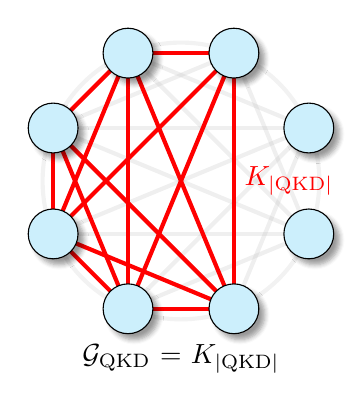
\begin{tikzpicture}[every node/.style={circle, draw, minimum size=1.8em, text width=1em, align=center, inner sep=0pt}, >=latex,
    myshadow/.style={
        blur shadow={shadow blur steps=5}
    }
]
    \def\UVsep{2.5em}
    \def\colSep{3em}
    \def\rowSep{1.2em}
    \def\hStep{0.7em}

    \definecolor{verylightgray}{rgb}{0.9, 0.9, 0.9}
    \colorlet{verylightorange}{orange!20}
    \colorlet{verylightblue}{cyan!20}

 % Radius of the circle
  \def\radius{5em}
  \def\numnodes{8}
  \def\degree{360/\numnodes}

  % Draw dummy nodes
  \foreach \x in {1,...,\numnodes} {
        \node[draw=none] (node\x) at (\x*\degree+0.5*\degree+180:\radius) {};
  }

  % Draw gray lines
  \foreach \x in {1,...,\numnodes} {
    \foreach \y in {\x,...,\numnodes} {
      \pgfmathparse{(\y>\x+1) && (1-(\x==1 && \y==\numnodes)) ? 1 : 0}
        \ifnum \pgfmathresult=1
            \draw[-,lightgray, opacity=0.25,line width=1.5,line cap=round] (node\x) -- (node\y);
        \fi
    }
  }
 \node[draw, circle, minimum size=2*\radius,verylightgray, opacity=0.5,line width=1.5,line cap=round] at (0,0) {};

  % Draw red lines
  \draw[-,red,line width=1.5,line cap=round] (node1) -- (node2);
  \draw[-,red,line width=1.5,line cap=round] (node1) -- (node5);
  \draw[-,red,line width=1.5,line cap=round] (node1) -- (node6);
  \draw[-,red,line width=1.5,line cap=round] (node1) -- (node7);
  \draw[-,red,line width=1.5,line cap=round] (node1) -- (node8);
  \draw[-,red,line width=1.5,line cap=round] (node2) -- (node5);
  \draw[-,red,line width=1.5,line cap=round] (node2) -- (node6);
  \draw[-,red,line width=1.5,line cap=round] (node2) -- (node7);
  \draw[-,red,line width=1.5,line cap=round] (node2) -- (node8);
  \draw[-,red,line width=1.5,line cap=round] (node5) -- (node6);
%  \draw[-,red,line width=1.5,line cap=round] (node5) -- (node7);
  \draw[-,red,line width=1.5,line cap=round] (node5) -- (node8);
  \draw[-,red,line width=1.5,line cap=round] (node6) -- (node7);
  \draw[-,red,line width=1.5,line cap=round] (node6) -- (node8);
  \draw[-,red,line width=1.5,line cap=round] (node7) -- (node8);

  % Visible nodes
  \foreach \x in {1,...,\numnodes} {
    \ifnum\x=1
        \node[circle,fill=verylightblue,myshadow] (node\x) at (\x*\degree+0.5*\degree+180:\radius) {};
    \else
       \ifnum\x=2
            \node[circle,fill=verylightblue,myshadow] (node\x) at (\x*\degree+0.5*\degree+180:\radius) {};
        \else
            \node[circle,fill=verylightblue,myshadow] (node\x) at (\x*\degree+0.5*\degree+180:\radius) {};
        \fi
    \fi
  }

  % Labels
  \coordinate (midK) at ($(node3)!0.5!(node4)$);
  \node[draw=none, left=0.9em of midK,text=red]
    {$K_{|\mathrm{QKD}|}$};
   
  \coordinate (mid) at ($(node1.east)!0.5!(node2.west) + (0,-1.8em)$); 
  \node[draw=none, rectangle, text width=8em] () at (mid) {$\mathcal{G}_\mathrm{QKD}=K_{|\mathrm{QKD}|}$};
\end{tikzpicture}
}
\hfill
\resizebox{0.49\columnwidth}{!}{
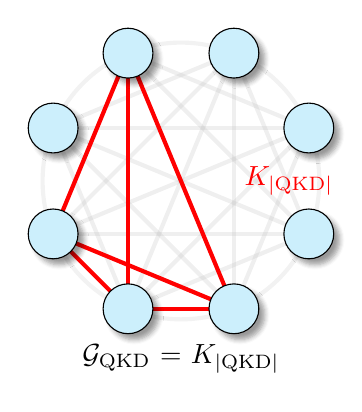
\begin{tikzpicture}[every node/.style={circle, draw, minimum size=1.8em, text width=1em, align=center, inner sep=0pt}, >=latex,
    myshadow/.style={
        blur shadow={shadow blur steps=5}
    }
]
    \def\UVsep{2.5em}
    \def\colSep{3em}
    \def\rowSep{1.2em}
    \def\hStep{0.7em}

    \definecolor{verylightgray}{rgb}{0.9, 0.9, 0.9}
    \colorlet{verylightorange}{orange!20}
    \colorlet{verylightblue}{cyan!20}

 % Radius of the circle
  \def\radius{5em}
  \def\numnodes{8}
  \def\degree{360/\numnodes}

  % Draw dummy nodes
  \foreach \x in {1,...,\numnodes} {
        \node[draw=none] (node\x) at (\x*\degree+0.5*\degree+180:\radius) {};
  }

  % Draw gray lines
  \foreach \x in {1,...,\numnodes} {
    \foreach \y in {\x,...,\numnodes} {
      \pgfmathparse{(\y>\x+1) && (1-(\x==1 && \y==\numnodes)) ? 1 : 0}
        \ifnum \pgfmathresult=1
            \draw[-,lightgray, opacity=0.25,line width=1.5,line cap=round] (node\x) -- (node\y);
        \fi
    }
  }
 \node[draw, circle, minimum size=2*\radius,verylightgray, opacity=0.5,line width=1.5,line cap=round] at (0,0) {};

  % Draw red lines
  \draw[-,red,line width=1.5,line cap=round] (node1) -- (node2);
%  \draw[-,red,line width=1.5,line cap=round] (node1) -- (node5);
  \draw[-,red,line width=1.5,line cap=round] (node1) -- (node6);
%  \draw[-,red,line width=1.5,line cap=round] (node1) -- (node7);
  \draw[-,red,line width=1.5,line cap=round] (node1) -- (node8);
%  \draw[-,red,line width=1.5,line cap=round] (node2) -- (node5);
  \draw[-,red,line width=1.5,line cap=round] (node2) -- (node6);
%  \draw[-,red,line width=1.5,line cap=round] (node2) -- (node7);
  \draw[-,red,line width=1.5,line cap=round] (node2) -- (node8);
%  \draw[-,red,line width=1.5,line cap=round] (node5) -- (node6);
%  \draw[-,red,line width=1.5,line cap=round] (node5) -- (node7);
%  \draw[-,red,line width=1.5,line cap=round] (node5) -- (node8);
%  \draw[-,red,line width=1.5,line cap=round] (node6) -- (node7);
  \draw[-,red,line width=1.5,line cap=round] (node6) -- (node8);
%  \draw[-,red,line width=1.5,line cap=round] (node7) -- (node8);

  % Visible nodes
  \foreach \x in {1,...,\numnodes} {
    \ifnum\x=1
        \node[circle,fill=verylightblue,myshadow] (node\x) at (\x*\degree+0.5*\degree+180:\radius) {};
    \else
       \ifnum\x=2
            \node[circle,fill=verylightblue,myshadow] (node\x) at (\x*\degree+0.5*\degree+180:\radius) {};
        \else
            \node[circle,fill=verylightblue,myshadow] (node\x) at (\x*\degree+0.5*\degree+180:\radius) {};
        \fi
    \fi
  }

  % Labels
  \coordinate (midK) at ($(node3)!0.5!(node4)$);
  \node[draw=none, left=0.9em of midK,text=red]
    {$K_{|\mathrm{QKD}|}$};
   
  \coordinate (mid) at ($(node1.east)!0.5!(node2.west) + (0,-1.8em)$); 
  \node[draw=none, rectangle, text width=8em] () at (mid) {$\mathcal{G}_\mathrm{QKD}=K_{|\mathrm{QKD}|}$};
\end{tikzpicture}
}
	%	\includegraphics[width=\columnwidth]{figures/proof_chains_QKD.pdf}	
	\caption{\textbf{QKD proof-chain for shared quantum randomness.} Amongst $n$ nodes with full $O(n^2)$ quantum communications connectivity given by the complete graph $K_n$, every node executes a QKD protocol with every other node, associating a shared random bit-string $s_{i,j}$ (received by $i$ from $j$) with every edge. Bit-strings passing a QRN certification function $f_\mathrm{QKD}(s_{i,j})$ define the edges of a subgraph, where certification acts as an implied vote of honesty. Maintaining only vertices connected to a majority of other nodes followed by eliminating those not connected to every other, we obtain a complete subgraph $\mathcal{G}_\mathrm{QKD}$ reflecting the unanimous majority.} \label{fig:proof_chains_QKD}
\end{figure}

\subsection{Consensus protocol} \label{sec:QRNG_consensus_protocol}

Associating QKD bit-strings $s_{i,j}$ with graph edges we assume a certification function,
\begin{align} \label{eq:QKD_verif}
	f_\mathrm{QKD}(s_{i,j})\to \{0,1\},
\end{align}
which evaluates \texttt{true} if $s_{i,j}$ passes a certification test for randomness. We define a QKD compliance graph with edge-inclusion based on the validity of the respective QKD bit-strings,
\begin{align}
	\mathcal{G}_\mathrm{QKD}^{(\mathrm{comp})}: e_{i,j} = f_\mathrm{QKD}(s_{i,j}).
\end{align}
Letting the QKD compliance of nodes be,
\begin{align} \label{eq:QKD_node_comp}
	\mathcal{G}_\mathrm{QKD}^{(\mathrm{comp})}: v_i = \textsc{Majority}\left(\bigcup_{j\neq i} e_{i,j}\right),
\end{align}
the reduced graph now only contains nodes whose associated QKD bit-strings $s_{i,j}$ are majority valid.

Additionally requiring unanimity demands finding a fully-connected subgraph, or clique\footnote{While the \textsc{MaxClique} problem of finding the largest cliques in a graph is known to be \textbf{NP}-complete in general, here we are not finding maximal cliques, affording an efficient solution.}, achieved by eliminating all vertices in $\mathcal{G}_\mathrm{QKD}^{\mathrm{(comp)}}$ not connected by an edge to every other node,
\begin{align}
	\mathcal{G}_\mathrm{QKD}: v_i =
	\begin{cases}
		1 & \text{if } |u_i \in \mathcal{G}_\mathrm{QKD}^{\mathrm{(comp)}}| = |\mathcal{G}_\mathrm{QKD}^{\mathrm{(comp)}}| - 1 \\
		0 & \text{otherwise}
	\end{cases}.
\end{align}
The fully connected \mbox{$\mathcal{G}_\mathrm{QKD}= K_{|\mathcal{G}_\mathrm{QKD}|}$} subgraph now represents the accepted subset of QKD-compliant nodes under consensus. The associated collectively established shared random bit-string is defined as,
\begin{align}
	s(\mathcal{G}_\mathrm{QKD}) = \bigoplus_{v_i,v_j\in \mathcal{G}_\mathrm{QKD}} {s_{i,j}}.
\end{align}

Although nodes could commit post-processed QKD strings obtained following post-selection and privacy amplification, this requires interaction between respective nodes. In the interests of maintaining a broadcast-only communications interface nodes may simply commit their raw unprocessed strings ($b$ and $m$) from which the associated QRNs $s$ are implied under a network-agreed post-processing function $f_\mathrm{PP}(\vec{b},\vec{m})\to \vec{s}$.

\section{Interactive proofs of quantumness} \label{sec:IPQ}

%\begin{figure}[!htb]
%	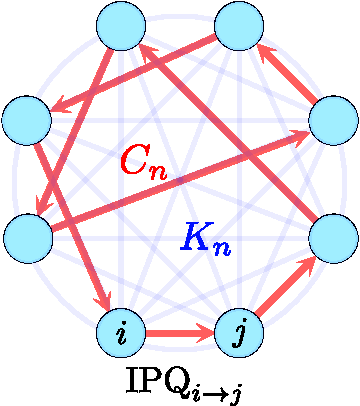
\includegraphics[width=0.35\columnwidth]{figures/proof_chains_IPQ.pdf}	
%	\caption{Proof-chain for shared quantum randomness. Amongst $n$ nodes with full quantum communications connectivity given by the complete graph $K_n$, nodes are randomly assigned to a cyclic graph $C_n\subseteq K_n$. Edges $e_{i,j}$ represent the establishment of shared quantum-random bit-strings between nodes. For entanglement-based (E91) randomness edges are undirected as the protocol is symmetric between $i$ and $j$. For BB84- and prover/verifier-based protocols nodes roles are asymmetric and edges are directed.} \label{fig:proof_chains_IPQ}
%\end{figure}

%Requiring all nodes to act as both prover and verifier once implies all vertices have in-degree and out-degree of 1,
%\begin{align}
%	\mathrm{deg}(v) = \mathrm{deg}(v) = 1\,\,\forall\,v\in V.
%\end{align}
%This implies the prover-verifier graph is a sum of disjoint cyclic graphs spanning all all nodes $v\in V$,
%\begin{align}
%	G_n = \sum_{\sum_i n_i = n} C_{n_i}	
%\end{align}

%If $G_n$ is the directed verifier graph the converse graph $G_n^\top$ represents the prover graph.
%
%Shared quantum-randomness requires only that a single QKD exchange be honest. i.e a single prover must be engaged honestly.

An interactive proof of quantumness \cite{Liu22, Zhu23} comprises two parties, a \emph{prover} and a \emph{verifier}, where the goal is for the prover to prove to the verifier that they have honestly executed a quantum implementation of some function $f(\cdot)$ that cannot be spoofed by classical simulation. The verifier has only classical resources and both parties may classically communicate.

While such protocols are not known in general for arbitrary $f(\cdot)$, they have been described in the context of a restricted class of functions known as trapdoor claw-free functions.

\subsection{Trapdoor claw-free (TCF) functions}

Trapdoor claw-free functions (TCF) are a class of cryptographic, 2-to-1, one-way functions,
\begin{align}
	f_\mathcal{I}(x)\to w,
\end{align}
which are classically efficient to evaluate in the forward direction, but for which it is hard to find simultaneously satisfying inputs $\{x_0,x_1\}$ (the `claw') mapping to the same output,
\begin{align}
	f(x_0)=f(x_1)=w,
\end{align}
where $x\in \{0,1\}^n$ and $w\in\{0,1\}^{n-1}$ are bit-strings.

Here, $\mathcal{I}$ denotes a problem instance derived from a secret (the trapdoor). If the secret is known, finding claws $\{x_0,x_1\}$ is classically efficient for any $w$. Since $f(\cdot)$ is easy to evaluate in the forward direction, verifying solutions is classically efficient, and the problem of  claw-finding by definition resides in the complexity class \textbf{NP}. %However, since inverting the trapdoor is hard the problem lies outside of the complexity class \textbf{P}, and outside \textbf{BQP} for post-quantum trapdoor functions.

%For an interactive proof of quantumness we desire claw-finding to be post-quantum and reside outside \textbf{BQP} such that a quantum prover is unable to spoof solutions by compromising the cryptographic integrity of $f(\cdot)$.

\subsection{The LWE problem}

A candidate TCF is the lattice-based learning with errors (LWE) problem \cite{Goldwasser85, Regev09, Regev10}. This problem is believed to be post-quantum, where the associated claw-finding problem lies outside of \textbf{BQP}, the class of problems efficiently solvable by quantum computers\footnote{An alternate number-theoretic TCF based on Rabin's function has been described \cite{Rabin79, Goldwasser88}. Since here the complexity of inverting the trapdoor reduces to integer factorisation this candidate TCF is vulnerable to quantum attack via Shor's algorithm \cite{Shor97}, making it less applicable in the assumed context of universal quantum computation.}.

For matrix,
\begin{align}
	A\in\mathbb{Z}_q^{m\times n},
\end{align}
and vectors,
\begin{align}
	x,y,s,e\in\{0,1\}^n,
\end{align}
related by,
\begin{align}
	y = A\cdot s + e,
\end{align}
under modulo $q$ arithmetic where $q$ is prime, a TCF may be constructed as,
\begin{align}
	f_\mathcal{I}(b,x_b) & = \lfloor A\cdot x + b\cdot y\rceil,
\end{align}
where $b=\{0,1\}$ is a single bit and claws are related by,
\begin{align}
	x_0=x_1+s.
\end{align}
Here, $\mathcal{I}=\{A,y\}$ specifies the problem instance derived from the secret trapdoor $\mathcal{T}=\{s,e\}$ secretly held by the verifier, enabling efficient classical claw-finding and verification if known.

Since $f(x)\to w$ is classically efficient to evaluate in the forward direction, it is easy to find a $w$ for which a single satisfying input $x$ is known. The challenge lies in finding simultaneously satisfying pairs of inputs, believed to be hard for both classical and quantum computers.

\subsection{Interactive proof protocol}

Taking a cryptographic TCF function, $f_\mathcal{I}(x)\to w$, an interactive proof of quantumness may be implemented as follows:

\begin{enumerate}
	\item The verifier specifies a problem instance $\mathcal{I}$, without revealing the associated secret $\mathcal{T}$ from which it was derived.
	\item The prover prepares a uniform superposition of all length-$n$ bit-strings $x$ via a Hadamard transform,
	      \begin{align}
		      \ket{\psi_H} & = \hat{H}^{\otimes n} \ket{0}^{\otimes n} = \frac{1}{\sqrt{2^n}} \sum_{x\in\{0,1\}^n} \ket{x}.
	      \end{align}
	\item Evaluating $f_\mathcal{I}(x)$ into an output register yields\footnote{The unitarity of quantum circuits prohibits direct evaluation of classical functions on quantum registers in general,
		      \begin{align}
			      \hat{U}_f\ket{x}\not\to\ket{f(x)},\nonumber
		      \end{align}
		      where $\hat{U}_f$ denotes a quantum circuit evaluating classical function $f(\cdot)$. Introducing ancillary quantum register $\ket{y}$ affords the reversible classical transformation $(x,y)\leftrightarrow(x,y\oplus f(x))$, which may be implemented unitarily in general,
		      \begin{align}
			      \hat{U}_f\ket{x}\ket{y}\to\ket{x}\ket{y\oplus f(x)}.\nonumber
		      \end{align}
		      Considering a single output bit of $f(\cdot)$, $\hat{U}_f$ admits the decomposition,
		      \begin{align}
			      \hat{U}_f = \hat\Pi_0\otimes \hat{I} + \hat\Pi_1\otimes \hat{X},\nonumber
		      \end{align}
		      where,
		      \begin{align}
			      \hat\Pi_i = \sum_{x\,|\,f(x)=i}\ket{x}\bra{x},\nonumber
		      \end{align}
		      are projectors onto the subspaces of $x$ satisfying \mbox{$f(x)=i$} (Nb: \mbox{$\hat\Pi_0+\hat\Pi_1=\hat{I}$}, \mbox{$\hat\Pi_0\cdot\hat\Pi_1=0$}). The unitarity of $\hat{U}_f$ follows, independent of $f(\cdot)$,
		      \begin{align}
			      \hat{U}_f^\dag \cdot \hat{U}_f & = (\hat\Pi_{0}\otimes \hat{I} + \hat\Pi_1\otimes \hat{X})^2 = \hat{I}.\nonumber
		      \end{align}
		      Repeating for all output bits and letting \mbox{$y=0$} yields,
		      \begin{align}
			      \hat{U}_f\ket{x}\ket{0}\to\ket{x}\ket{f(x)}.\nonumber
		      \end{align}},
	      \begin{align}
		      \ket{\psi_\mathcal{I}} & = \frac{1}{\sqrt{2^n}} \sum_{x\in\{0,1\}^n} \ket{x} \ket{f_\mathcal{I}(x)},\nonumber
	      \end{align}
	      which may be efficiently prepared using a quantum circuit with,
	      \begin{align}
		      O(n^2 \log^2 n),
	      \end{align}
	      gate count \cite{ClassVerifQA}.
	\item The prover measures the output register, obtaining measurement outcome $w$ which is communicated to the verifier. Measuring $w$ collapses the $x$-register onto the equal superposition of associated satisfying pre-images,
	      \begin{align}
		      \ket{\psi_w} = \frac{1}{\sqrt{2}}(\ket{x_0}+\ket{x_1})\ket{w}.
	      \end{align}
	      As the $x$-register was initialised into a uniform superposition over all length-$n$ bit-strings and the TCF is a 2-to-1 function, $w$ is sampled uniformly at random.
	\item The verifier specifies a random measurement basis in which the prover should measure qubits in the $x$ register, where $b=\{0\equiv \hat{Z},1\equiv\hat{X} \}$ correspond to the respective Pauli measurement bases.
	\item When measuring in the $b=0$ ($\hat{Z}$) basis, the prover randomly measures either $m=x_0$ or $m=x_1$, easily verified by direct evaluation of \mbox{$f(x)\to w$} and comparison with the prover's previously reported $w$. When measuring in the $b=1$ ($\hat{X}$) basis verification succeeds if \mbox{$m\cdot x_0 = m\cdot x_1$}. The verification rules are,
	      \begin{align}
		      \hat{Z}\, (b=0): & \quad m=\{x_0,x_1\},\nonumber  \\
		      \hat{X}\, (b=1): & \quad m\cdot x_0 = m\cdot x_1.
	      \end{align}
	\item The above is repeated some constant number of rounds, independently randomising the measurement basis $b$ at every round.
\end{enumerate}

The key observation is that since $\hat{X}$ and $\hat{Z}$ measurements do not commute, it is not possible for the prover to know both measurement outcomes simultaneously and therefore must measure in accordance with the verifier's stated measurement basis to pass verification of a single round. While a single round can be classically spoofed if the measurement basis $b$ is known in advance of announcing $w$, if unknown, $b$ can only be guessed with a probability of $1/2$. Upon repetition, the probability of correctly guessing all measurement bases scales as \mbox{$p=1/2^n$} for $n$ rounds, ensuring asymptotic confidence in the honesty of the prover.

\subsection{Consensus protocol}

To incorporate IPQs into the QCN framework we require all nodes to act as both prover and verifier for all other nodes.

In the verifier capacity every node prepares a single random TCF instance for all other nodes to prove. Despite solving the same problem instance their proofs will be distinct.

Following the same approach as with QKD we represent the proofs-of-quantumness via a complete graph with the distinction that as this is an asymmetric protocol the graph is now directed (from prover to verifier) with edges in both directions for every node-pair.

Majority votes as per Eq.~\eqref{eq:QKD_node_comp} are now made from the verifier perspective.

The additional synchronous steps required to accommodate IPQs are:
\begin{enumerate}
	\item Nodes commit a single random problem instance $\mathcal{I}_i$.
	\item Nodes execute the quantum problem instance specified by every other node $j$ and commit the obtained $w_{i,j}$.
	\item Nodes commit the random measurement bases $b_i$ other nodes will be required to measure in.
	\item Nodes complete their quantum computations and commit the obtained measurements $m_{i,j}$.
	\item Nodes reveal their secrets $\mathcal{T}_i$.
\end{enumerate}

Assuming a verification function analogous to Eq.~\eqref{eq:QKD_verif},
\begin{align}
	f_\mathrm{IPQ}(\mathcal{I}_i,\mathcal{T}_i,w_{i,j},b_i,m_{i,j}) \to \{0,1\},
\end{align}
similarly defines a directed IPQ compliance graph,
\begin{align}
	G_\mathrm{IPQ}^{\mathrm{comp}}: e_{i,j} = f_\mathrm{IPQ}(\mathcal{I}_i,\mathcal{T}_i,w_{i,j},b_i,m_{i,j}) \to \{0,1\}.
\end{align}

%A classical cheater can spoof a single round of this protocol if the measurement basis is known in advance. For example, if known that the measurement basis will be $Z$, they can choose a random $x$, efficiently evaluate $f(x)\to w$ in the forward direction, and pass the $Z$ test. However, if $b$ is chosen at random, they will only be able to do this half the time if the full claw is not known. 

%
%The full proof for a multi-round implementation of this protocol between provers ($i\in\mathcal{S}_P$) and verifiers ($j\in\mathcal{S}_V$) is given by,
%\begin{align}
%	\mathcal{P}_{i,j} = \{\mathcal{I}_j,\{w_{i,j}^{(k)}\},\{b_{j}^{(k)}\},\{m_{i,j}^{(k)}\}\},
%\end{align}
%where $0\leq k < N_R$ indexes the round.

%\section{QIP}
%
%From the proof system, $\mathcal{P}_S$, we define the node keys,
%\begin{align}
%	k_i &= \bigoplus_{j,k} w_{i,j}^{(k)},
%\end{align}
%for each prover $i\in\mathcal{S}_P$, and a collective key,
%\begin{align}
%	k &= \bigoplus_i k_i,
%\end{align}
%which is guaranteed to be quantum-random if at least one proof was honest and obtained via quantum computation. Under the action of the bitwise XOR operation on the set $\{k_i\}$, $k$ implements a random permutation $\sigma\in S_{|\mathcal{S}_P|}$ on the ordering of the set of provers $\mathcal{S}_P$ ,
%\begin{align}
%k \oplus \{k_i\} \cong \sigma(\mathcal{S}_P),
%\end{align}
%where $\sigma\in S_{|\mathcal{S}_P|}$ denotes a permutation in the symmetric group over $|\mathcal{S}_P|$ elements.
%
%Exploiting this property, for each prover we define the permuted key,
%\begin{align}
%	\tilde{k}_i &= k \oplus k_i	= \bigoplus_{j\neq i} k_j,
%\end{align}
%which cannot be manipulated as $k$ is not known prior to commitment of $\{k_i\}$.
%
%Ordering provers by $\tilde{k}_i$ creates a quantum randomly ordered set. Upon piecewise partitioning we obtain non-intersecting random subsets, all perfect quantum-random solutions to the random subset problem, assuming at least one honest proof.


\bibliography{bibliography}

\end{document}
